\subsection{RemotePeerMeter}\label{sec:mit-peer-meter}
Based on the \lstinline|RemotePeerMeter| the \lstinline|PeerManager| gathers information about the quality of a \lstinline|RemotePeer|. The quality of a peer is needed for the candidate selection to transmit a message.
Besides the quality the RemotePeerMeter also provides some other metrics that are presented in \vref{fig:mit-remote-peer-meter} and further described in this section.

\begin{figure}
\centering
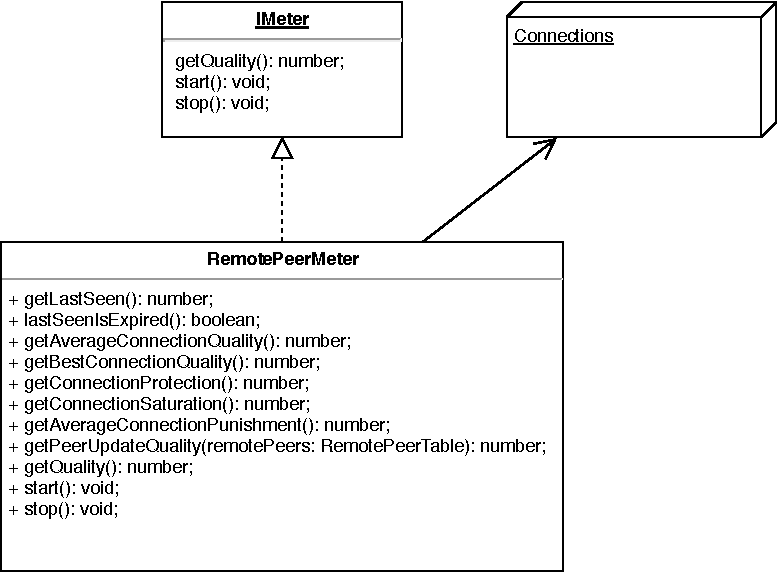
\includegraphics[width=0.75\textwidth]{graphics/implementation/mitosis-architecture-PeerMeter.pdf}
\caption{RemotePeerMeter}
\label{fig:mit-remote-peer-meter}
\end{figure}

\paragraph{LastSeen}
\lstinline|LastSeen| is a metric that represents the vitality of a peer. Each time a message is received from a RemotePeer its last seen tick is set to the current tick. The longer the RemotePeer has not send a message the older is its LastSeen. When it exceeds a certain threshold the RemotePeer is seen as crashed and therefor removed. 
As a remote peer can have multiple connections the LastSeen metric is based on the youngest LastSeen of all connections (\vref{lst:mit-last-seen}). Youngest means a more recent LastSeen.

Whether the Peer is seen as crashed is determined by the delta value of the current application tick and the youngest last seen (\vref{lst:mit-crashed}).

\paragraph{Connection Quality}
The connection is responsible to measure its quality to a RemotePeer. Each connection type has its own mechanism how to do so. This is further explained in \vref{sec:mit-connectionMeter}.
The RemotePeerMeter can determine the average connection quality (\vref{lst:mit-average-connection-quality}) and the best available connection quality (\vref{lst:mit-best-connection-quality}.

\paragraph{RemotePeer Newcomer Protection}
When a connection to a new RemotePeer is established the \textit{Newcomer Protection} becomes active as long as the new peer does not have any other connections. This prevents that the new RemotePeer might be kicked out immediately because of the peer desire to achieve its own connection goal. The Newcomer Protection is active for a global defined time window or when the other peer has managed to establish connections to other peers (\vref{lst:mit-welpenschutz}).

\paragraph{Connection Saturation}
The connection saturation of a RemotePeer is calculated by counting all reported connections and the amount of direction connections. Each peer has the desire to obtain a certain amount of peers (default is $\ 5 $) but also a maximum limit of allowed connections (default is $\ 10 $). This applies for all peers, therefore a peer can derive how many free connections a remote peer has. \vref{fig:mit-remote-peer-saturation} shows a sample calculation and \vref{lst:mit-connection-saturation} the belonging pseudo code. 
However, this is just an estimation because a peer only knows the reports of direct peers. As seen in the \vref{fig:mit-remote-peer-saturation} \textit{Node D} is also connected to \textit{Node E}, but as \textit{Node A} does not have a direct connection to \textit{Node E}, it does not know about its existence.
The saturation value is limited to a value between $\ 0 $ and $\ 1 $. As long as the estimated connection is below the desired connection goal the value is $\ 0 $, otherwise a value between $\ 0 $ and $\ 1 $, where $\ 0 $ is a good probability and $\ 1 $ a bad one.
The saturation value is used when alternative RemotePeers are recommended to a peer, that is trying to connect but max connections are already reached.

\begin{figure}
\centering
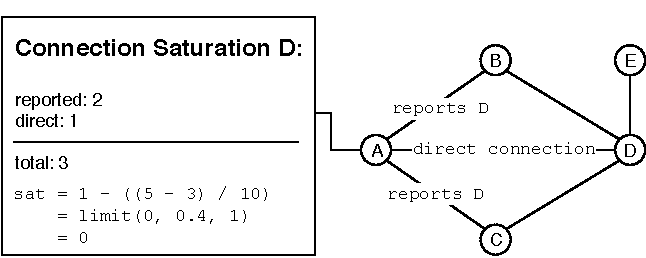
\includegraphics[width=0.75\textwidth]{graphics/implementation/mitosis-architecture-Connection-Saturation.pdf}
\caption{Peer A's calculation of RemotePeer D's Saturation }
\label{fig:mit-remote-peer-saturation}
\end{figure}

\paragraph{Connection Punishment}
A punishment for a connection is applied when it can not be successfully established within a global defined time window or is prematurely closed. The punishment shall ensure that the peer does not immediately retry to open a connection again. After a a globally specified timeout the punishment for a connection is revoked.
The RemotePeerMeter provides the metric of the average amount of punished connections. When a peer has a lot of punished connections it is less likely considered in the peer selection.

\paragraph{Report Quality}\label{par:mit-report-quality}
A peer is reporting its remote peers via a \peerUpdate, where each RemotePeer has a quality. The quality is calculated by the best connection quality to remote peer and its connection saturation (\vref{lst:mit-remote-peer-quality-report}). Based on the reported quality in the \peerUpdate, the receiver can select the RemotePeer as a potential connection partner. 

\paragraph{RemotePeer Quality}
The RemotePeer quality is used during the selection process of the PeerManager for message delivery. The quality is derived by the average connection quality and a punishment factor (\vref{lst:mit-remote-peer-quality}). When a peer has a lot of punished connections it is considered as unstable and becomes less likely selected for the message delivery.

\paragraph{Router alive score}
Each RemotePeer is maintaining a router score, meaning that a peer who receives a router alive first gets a better rank than one that receives it later. A router alive comes with a sequence number. When the sequence number is unknown, the PeerManager adds a new sequence with an undefined rank for all directly connected RemotePeers. Afterwards the rank of the RemotePeer who has delivered the message is set to $\ 1 $.
When a router alive message is received where the sequence number is already known, the rank of the deliver peer is set to the amount of RemotePeers who have delivered it already.
The score is an average of the rank of all received sequence numbers. When a sequence number does not have a rank it is ignored.
The goal of the router alive score is to bring peers closer to the router. During the peer selection process, via-RemotePeers that have a better connection to a peer who knows the router are favored.